\section{Интерполирование кривой по набору точек и направлениям касательных}

\begin{figure}[h!]
\center{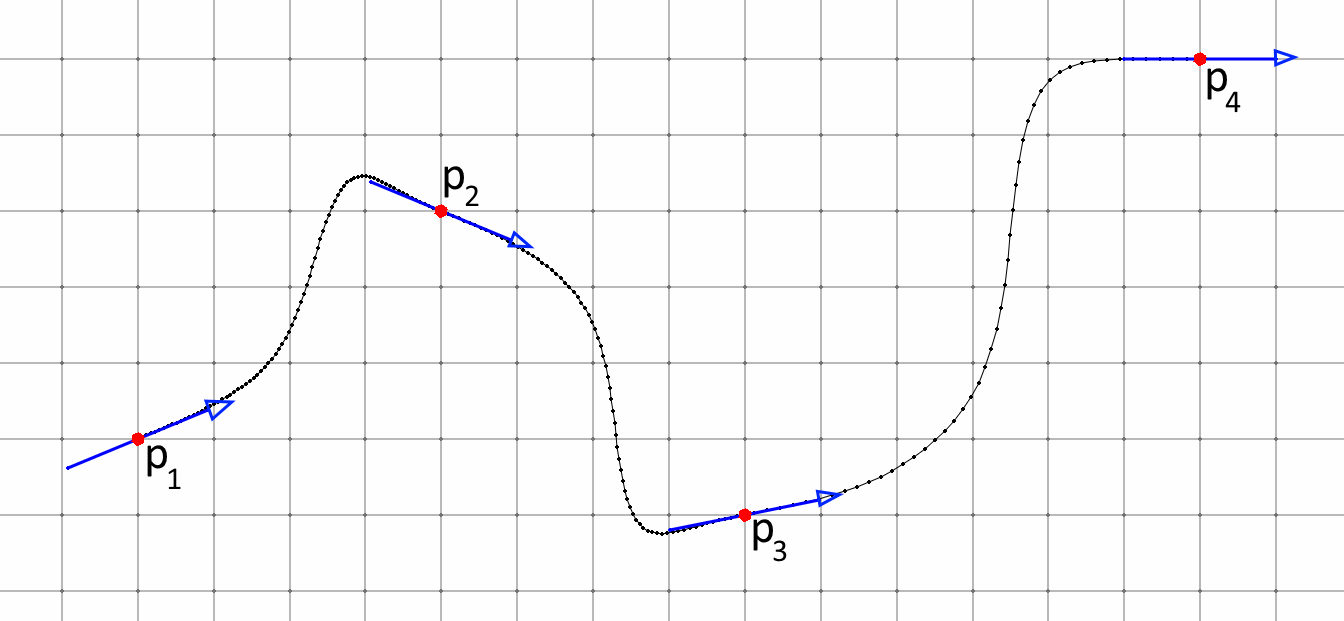
\includegraphics[scale=0.5]{by-tangents-plane}}
\caption{Интерполирование кривой по набору точек и направлениям касательных на плоскости}
\label{picture-by-tangents-plane}
\end{figure}

\begin{figure}[h!]
\center{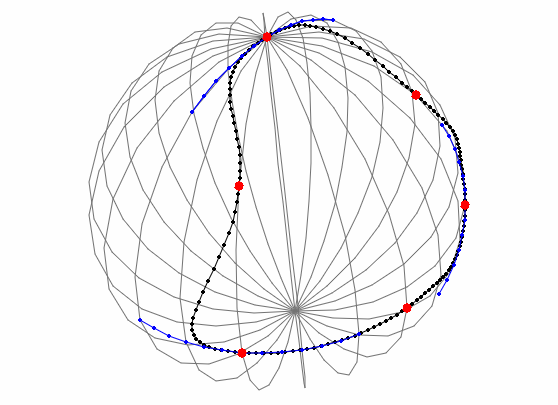
\includegraphics[scale=1.05]{by-tangents-two-dimension}}
\caption{Интерполирование кривой по набору точек и направлениям касательных на двумерной сфере}
\label{picture-by-tangents-two-dimension}
\end{figure}

На рис.~\ref{picture-by-tangents-plane} изображена сплайн-кривая на плоскости, построенная по набору точек и
направлениям касательных. В каждой точке $p_i$ задан угол к оси $Ox$, указанный стрелкой. Можно видеть, что
построенная кривая действительно проходит через точки $p_i$ под заданными углами.

На рис.~\ref{picture-by-tangents-two-dimension} изображена сплайн-кривая на поверхности двумерной сферы, построенная
по набору точек и направлениям касательных. Точки выбраны таким образом, чтобы кривая была замкнутой. Углы к экватору
заданы не во всех точках: там, где они заданы, можно видеть касательные дуги.

На рис.~\ref{picture-by-tangents-orientation} можно видеть набор ориентаций 3D-объекта, причём у трёх средних
ориентаций заданы углы к экватору. Чёрная кривая "--- это тот путь, который пройдёт самая верхняя точка объекта
при воспроизведении построенной анимации. Можно видеть, что объект действительно пройдёт через ориентации под
заданными углами.

\begin{figure}[h!]
\center{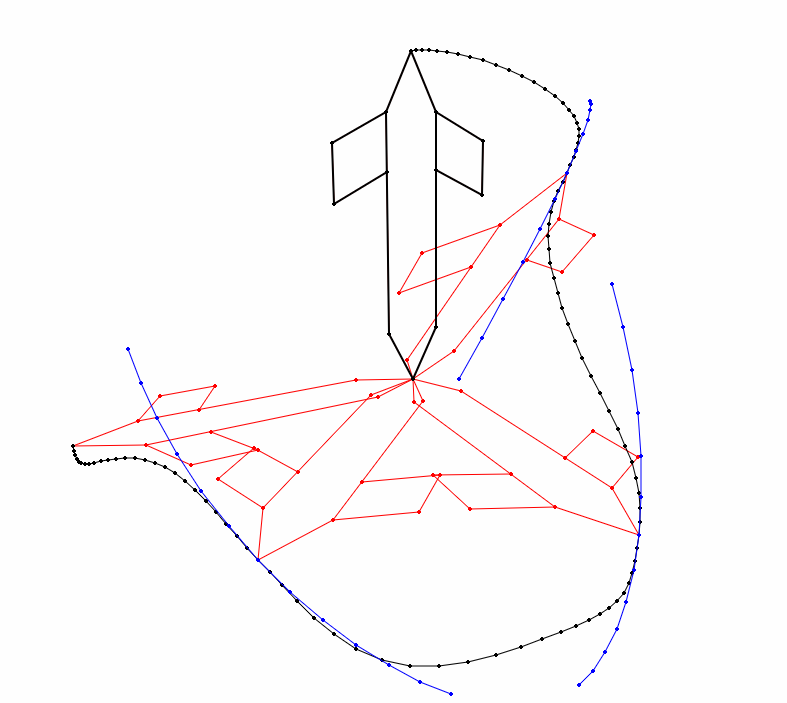
\includegraphics[scale=0.75]{by-tangents-orientation}}
\caption{Интерполирование кривой по набору точек и направлениям касательных на ориентационной сфере}
\label{picture-by-tangents-orientation}
\end{figure}
